\section{Meta-Learning}

% ---------------------------------------------------------------- Slide 8
\begin{frame}{What is meta-learning?}
\begin{columns}[c]
\begin{column}{0.62\textwidth}
\begin{itemize}
    \item If you've learned 100 tasks already, can you figure out how to learn more
          efficiently?
    \begin{itemize}\item Now having multiple tasks is a huge advantage!\end{itemize}
    \item Meta-learning $=$ learning to learn
    \item In practice, very closely related to multi-task learning
    \item Many formulations
    \begin{itemize}
        \item Learning an optimizer
        \item Learning an RNN that ingests experience
        \item Learning a representation
    \end{itemize}
\end{itemize}
\end{column}
\begin{column}{0.38\textwidth}
\centering
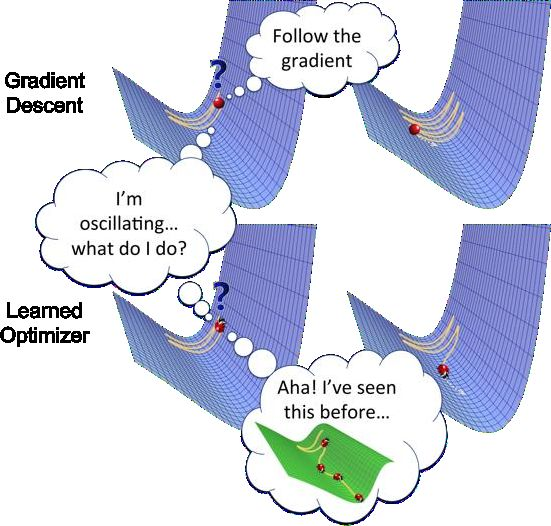
\includegraphics[width=\linewidth]{images/meta-rl-open/figures/meta-learn-bird.jpg}
\end{column}
\end{columns}
\end{frame}

% ---------------------------------------------------------------- Slide 9
\begin{frame}{Why is meta-learning a good idea?}
\begin{itemize}
    \item Deep reinforcement learning, especially model-free, requires a huge number of
          samples
    \item If we can meta-learn a faster reinforcement learner, we can learn new tasks
          efficiently!
    \item What can a meta-learned learner do differently?
    \begin{itemize}
        \item Explore more intelligently
        \item Avoid trying actions that are know to be useless
        \item Acquire the right features more quickly
    \end{itemize}
\end{itemize}
\end{frame}

% ---------------------------------------------------------------- Slide 10
\begin{frame}{Meta-learning with supervised learning}
\vfill
\centering
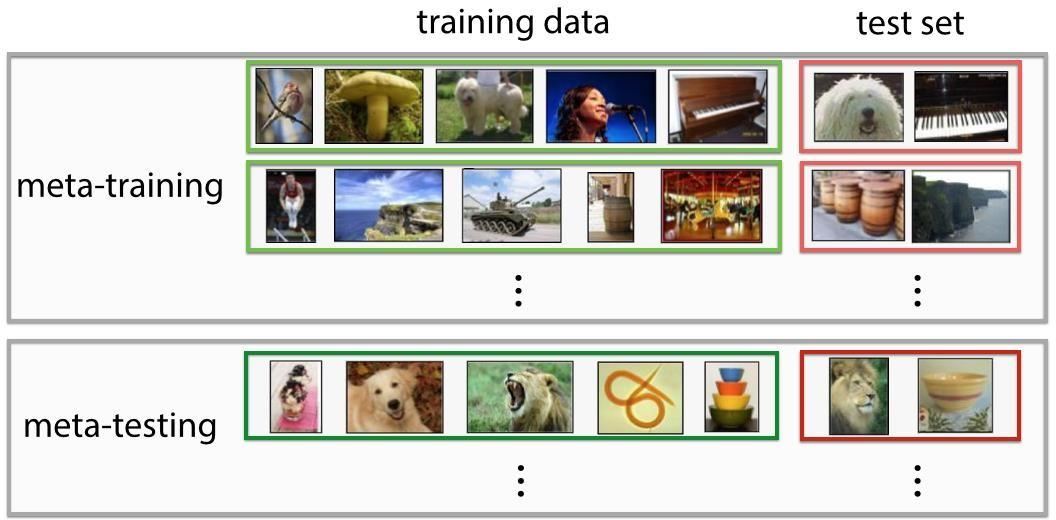
\includegraphics[width=0.85\linewidth]{images/meta-rl-open/figures/few-shot.jpg}
\vfill
{\scriptsize image credit: Ravi \& Larochelle '17}
\end{frame}

% ---------------------------------------------------------------- Slide 11
\begin{frame}{Meta-learning with supervised learning}
\begin{columns}[c]
\begin{column}{0.5\textwidth}
\centering
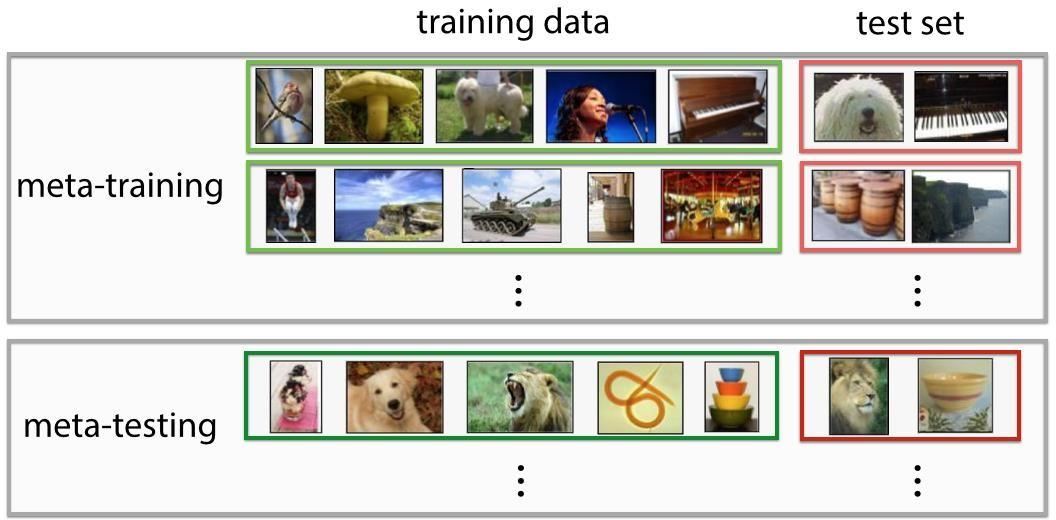
\includegraphics[width=\linewidth]{images/meta-rl-open/figures/few-shot.jpg}\\[0.6em]
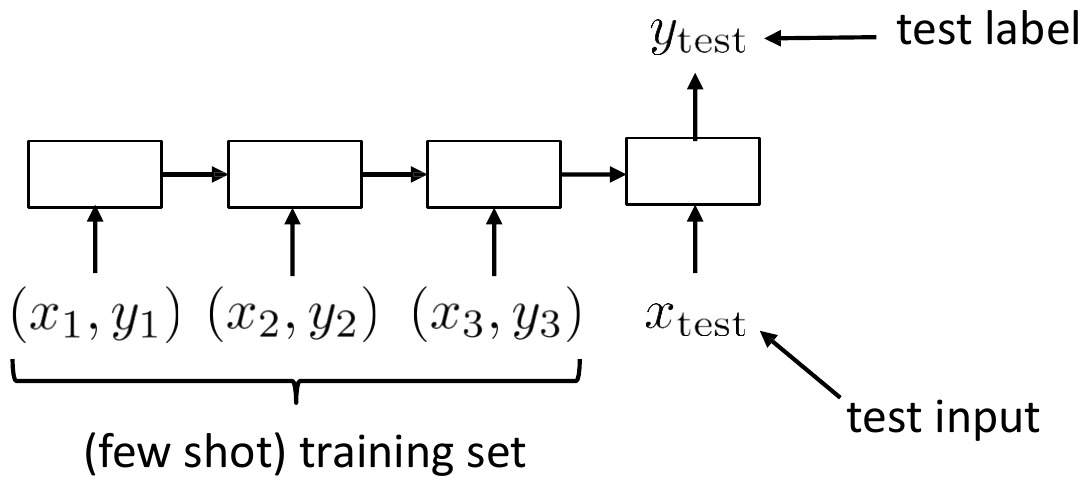
\includegraphics[width=0.95\linewidth]{images/meta-rl-open/figures/rnn-11.jpg}
\end{column}
\begin{column}{0.5\textwidth}
\centering
\resizebox{\linewidth}{!}{%
\begin{tikzpicture}[font=\small, inner sep=1pt,
    ar/.style={-{Stealth[length=1.6mm]}, shorten >=1pt}]
    \node (sl) {supervised learning:\; $f($};
    \node[right=0pt of sl] (x) {$x$};
    \node[right=0pt of x] (r1) {$) \rightarrow$};
    \node[right=2pt of r1] (y) {$y$};
    \node[below=0.9cm of x, font=\scriptsize, xshift=-1.0cm] (inp) {input (e.g., image)};
    \node[below=0.9cm of y, font=\scriptsize, xshift=1.2cm] (out) {output (e.g., label)};
    \draw[ar] (inp) -- (x);
    \draw[ar] (out) -- (y);
\end{tikzpicture}}

\vspace{1.4em}
\resizebox{\linewidth}{!}{%
\begin{tikzpicture}[font=\small, inner sep=1pt,
    ar/.style={-{Stealth[length=1.6mm]}, shorten >=1pt}]
    \node (ml) {supervised meta-learning:\; $f($};
    \node[right=0pt of ml] (D) {$\mathcal{D}^{\text{tr}}$};
    \node[right=0pt of D] (r2) {$,x) \rightarrow y$};
    \node[below=0.7cm of D, font=\scriptsize] (ts) {training set};
    \draw[ar] (ts) -- (D);
\end{tikzpicture}}

\vspace{1.0em}
\begin{itemize}
    \item How to read in training set?
    \begin{itemize}
        \item Many options, RNNs can work
        \item More on this later
    \end{itemize}
\end{itemize}
\end{column}
\end{columns}
\end{frame}

% ---------------------------------------------------------------- Slide 12
\begin{frame}{What is being ``learned''?}
\begin{columns}[c]
\begin{column}{0.55\textwidth}
\centering
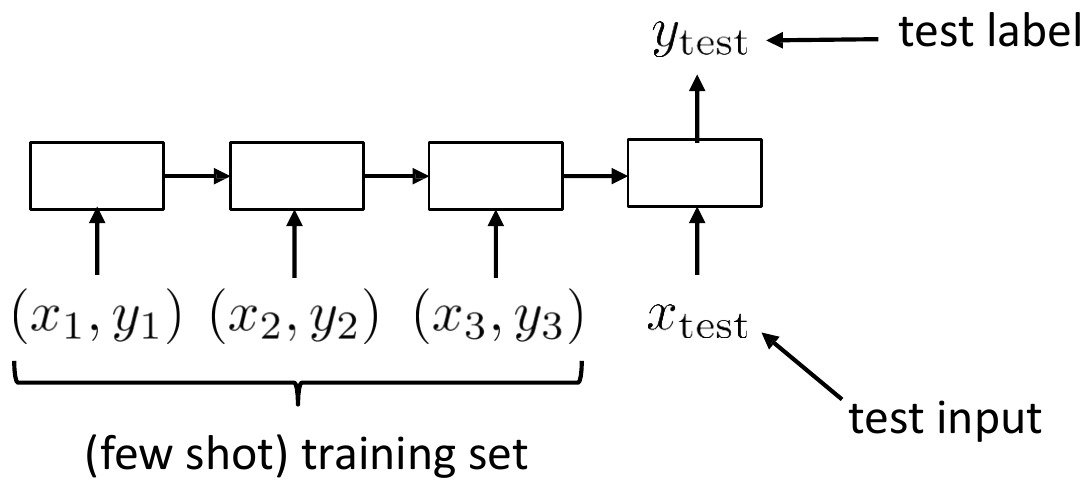
\includegraphics[width=\linewidth]{images/meta-rl-open/figures/rnn-12.jpg}
\end{column}
\begin{column}{0.45\textwidth}
supervised meta-learning:
\[ f(\mathcal{D}^{\text{tr}}, x) \rightarrow y \]
\end{column}
\end{columns}
\vfill
\begin{columns}[t]
\begin{column}{0.5\textwidth}
\centering\footnotesize ``Generic'' learning:
\begin{align*}
    \theta^\star &= \arg\min_\theta \mathcal{L}(\theta, \mathcal{D}^{\text{tr}})\\
    &= f_{\text{learn}}(\mathcal{D}^{\text{tr}})
\end{align*}
\end{column}
\begin{column}{0.5\textwidth}
\centering\footnotesize ``Generic'' meta-learning:
\begin{align*}
    \theta^\star &= \arg\min_\theta \sum_{i=1}^{n} \mathcal{L}\!\left(\phi_i, \mathcal{D}^{\text{ts}}_i\right)\\
    \text{where } \phi_i &= f_\theta(\mathcal{D}^{\text{tr}}_i)
\end{align*}
\end{column}
\end{columns}
\end{frame}

% ---------------------------------------------------------------- Slide 13
\begin{frame}{What is being ``learned''?}
\begin{columns}[t]
\begin{column}{0.5\textwidth}
\centering\footnotesize ``Generic'' learning:
\begin{align*}
    \theta^\star &= \arg\min_\theta \mathcal{L}(\theta, \mathcal{D}^{\text{tr}})\\
    &= f_{\text{learn}}(\mathcal{D}^{\text{tr}})
\end{align*}
\end{column}
\begin{column}{0.5\textwidth}
\centering\footnotesize ``Generic'' meta-learning:
\begin{align*}
    \theta^\star &= \arg\min_\theta \sum_{i=1}^{n} \mathcal{L}\!\left(\phi_i, \mathcal{D}^{\text{ts}}_i\right)\\
    \text{where } \phi_i &= f_\theta(\mathcal{D}^{\text{tr}}_i)
\end{align*}
\end{column}
\end{columns}
\vfill
\begin{columns}[c]
\begin{column}{0.55\textwidth}
\centering
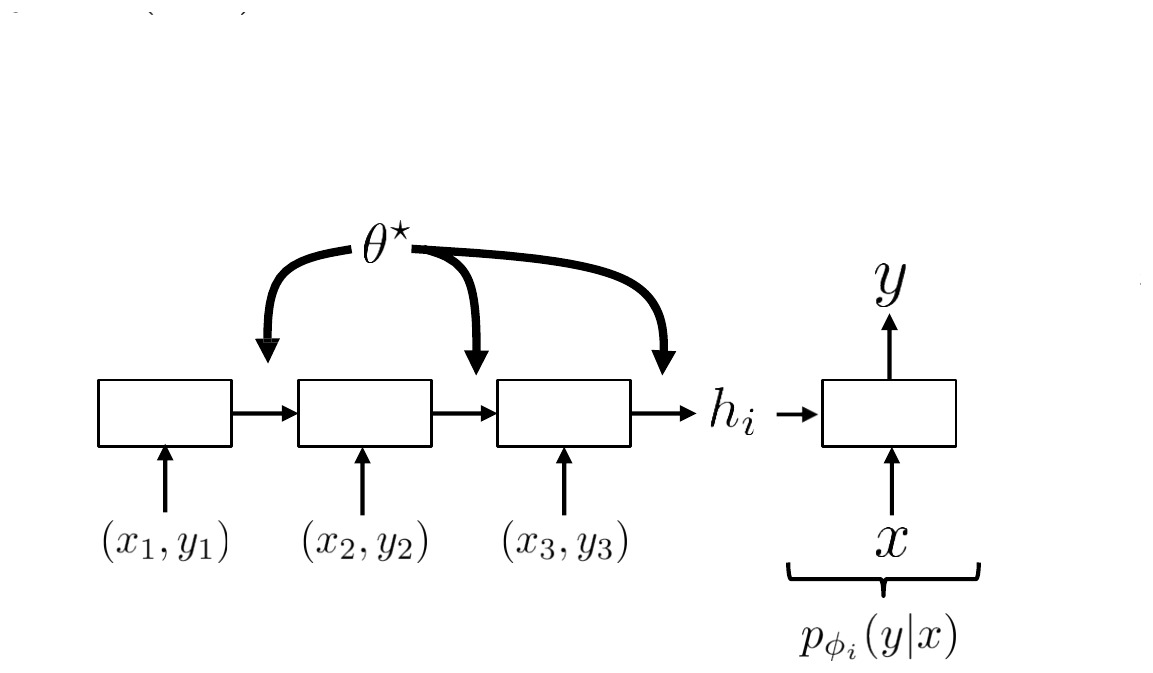
\includegraphics[width=\linewidth]{images/meta-rl-open/figures/rnn-13.jpg}
\end{column}
\begin{column}{0.45\textwidth}
\centering
\begin{tikzpicture}[inner sep=1pt, ar/.style={-{Stealth[length=1.8mm]}}]
    \node (phi) {$\phi_i = [\,$};
    \node[right=0pt of phi] (h) {$h_i$};
    \node[right=0pt of h] (cm) {$,\;$};
    \node[right=0pt of cm] (th) {$\theta_p$};
    \node[right=0pt of th] (rb) {$\,]$};
    \node[above=0.95cm of h, font=\scriptsize, align=center, xshift=-0.7cm] (rnnh) {RNN hidden\\ state};
    \node[above=0.95cm of th, font=\scriptsize, align=center, xshift=0.9cm] (mlw) {meta-learned\\ weights};
    \draw[ar] (rnnh) -- (h);
    \draw[ar] (mlw) -- (th);
\end{tikzpicture}
\end{column}
\end{columns}
\end{frame}
